i\chapter{Methodology}
\label{chap:methodology}
 
\section{Introduction}
This chapter highlights the different techniques that where used to successfully complete the project. It provides a consise description for the data collection and analysis methods, system design and implementation methods, together with the system testing and validation techniques that were applied to make sure that Traxis satisfies and meets user requirements.
\vspace{1cm}

The key phases to be undertaken where:

\begin{itemize}
    \item \textbf{Data Collection}: Comprehensive data on commuter needs, driver challenges, and existing platform functionalities was acquired through interviews, surveys and competitive analysis.
    
    \item \textbf{System Design and Implementation}: The  overall architecture, UI/UX, and core features were then designed, developed and implemented for the full Traxis system.
    
    \item \textbf{Testing and Validation}: Comprehensive functional, performance, and usability testing were done to ensure the system meets the specified requirements and performs reliably under real-world conditions.
    
\end{itemize}

\section{Data Collection}
This phase focused on systematically identifying and analyzing both functional and non-functional requirements for Traxis. The primary objective was to deeply understand commuter pain points, driver operational challenges, and gaps in existing transport platforms in the private taxi ecosystem ensuring that the final system is grounded in real world needs rather than assumptions.

\subsection{Data Collection Techniques}

\begin{itemize}

    \item \textbf{Semi-structured Interviews}: In-depth interviews with private shuttle coordinators, drivers, and frequent passengers were conducted to uncover coordination bottlenecks, safety concerns, trust issues, and desired digital interventions.
    
    \item \textbf{Questionnaires}: Targeted surveys were distributed to a broader passenger base (minimum target: 100  respondents) to quantify commuting patterns, smartphone penetration, willingness to adopt app-based solutions, and feature priorities.
    
    \item \textbf{Direct Observation}: Field observation at private shuttle stages was done to document real driver–passenger interactions, queue dynamics, information asymmetry, and operational inefficiencies that users may not articulate in interviews.
    
    \item \textbf{Competitive Analysis}: Evaluation of existing ride-hailing and transport apps operating in East Africa (e.g., Uber, Bolt, SafeBoda, digital matatu initiatives) was done to identify functional gaps and lessons applicable to the informal taxi sector.
\end{itemize}

\subsection{Tools and materials}

\begin{table}[h!]
\centering
\begin{tabular}{|l|l|}
\hline
\textbf{Data Collection Method} & \textbf{Tools and Materials} \\ \hline
Questionnaires & Pens and printed questionnaires; Google Forms \\ \hline
Interviews & Interview guide; Pens and notebooks; Smartphones \\ \hline
Observations & Smartphones \\ \hline
\end{tabular}
\caption{Tools and Materials Used for Data Collection}
\end{table}

\section{System Design and Implementation}

To ensure effective and well-coordinated project management, the Agile software development methodology was be adopted throughout the project lifecycle. This approach contributed significantly to the success of the project by enabling iterative planning, continuous evaluation, and timely adjustments to project activities. By anticipating the need for flexibility in time management and task execution, the team was able to respond efficiently to changing requirements, minimize potential delays, and maintain steady progress toward the project objectives.

\subsection{System Design}
The system was architected around two primary entities to guarantee reliable communication, scalability, data consistency, and overall operational efficiency across the platform.

\begin{itemize}
    \item \textbf{Clients}: Two dedicated mobile applications were deployed on the smartphones of passengers and drivers.  
    \textit{The Passenger Application and the Driver Application that functioned as client-side components, handling user interactions, location updates, and real-time requests while communicating securely with the backend services.}

    \item \textbf{Server} (Single Source of Truth): A centralized, cloud-hosted backend system that acted as the authoritative source for all application data and system state. The server was responsible for coordinating passenger–driver matching, enforcing business rules, synchronizing data across all connected clients, and maintaining consistency in real-time operations. Additionally, it handled secure data storage, backups, authentication, logging, and fault tolerance, ensuring data integrity, system reliability, and recoverability in the event of failures or network disruptions.
\end{itemize}

\subsubsection{Client Design}

The client application was be developed using \textbf{Dart}, a modern, object-oriented programming language developed by Google and optimized for building fast, scalable user interfaces. Dart was used in combination with the \textbf{Flutter} framework, which enabled cross-platform application development from a single codebase. This allowed the application to run on both Android and iOS platforms while reducing development time, simplifying maintenance, and ensuring a consistent user experience across devices.

The client-side design adopted a modular architecture, where each functional feature was implemented as an independent component. Flutter’s widget-based structure promoted reusability, scalability, and maintainability, while supporting responsive and adaptive user interfaces.

The client application integrated the following technologies:

\begin{itemize}
    \item \textbf{Firebase Authentication (Firestore Auth)} was used to manage user authentication and identity for both passengers and drivers. Firebase provided a secure and scalable platform for login, registration, and session management, allowing the development team to focus on core application functionality.
    
    \item \textbf{Firebase Cloud Messaging (FCM)} delivered real-time notifications such as ride requests, trip updates, and system alerts. FCM enabled reliable and low-latency push messaging across devices without requiring custom notification infrastructure.
    
    \item \textbf{Google Maps API} supported geolocation services, route visualization, distance calculations, and real-time location tracking. It provided a robust mapping platform that integrated seamlessly with mobile applications.
    
    \item \textbf{AWS Services} were used to implement transcription and other compute-intensive features. AWS (Amazon Web Services) offered scalable cloud-based computing resources, ensuring that tasks such as voice-to-text conversion were processed efficiently and reliably.
    
    \item \textbf{MCP (Model Control Plane)} was employed to enable AI-powered features implemented in \textbf{Python}, a high-level programming language well-suited for machine learning, data processing, and AI integration. MCP allowed the client to interact with intelligent services through well-defined APIs.
\end{itemize}

Overall, the client design prioritized responsiveness, scalability, and seamless integration with backend services while maintaining a clear separation between presentation logic and data handling.

\subsubsection{Server Design}

The server-side component was deployed on a \textbf{cloud-based infrastructure} to ensure scalability, high availability, and fault tolerance. The backend was implemented using \textbf{Django}, a high-level web framework built with \textbf{Python}, chosen for its simplicity, security, and rapid development capabilities.

Django served as the core framework responsible for processing client requests, handling business logic, managing API endpoints, and coordinating communication between clients and external services.

The server utilized \textbf{PostgreSQL}, an advanced open-source relational database, for all persistent data storage. PostgreSQL was known for its reliability, strong data integrity, support for complex queries, and transactional consistency, ensuring accurate management of user profiles, trip data, logs, and system metadata.

\textbf{Gunicorn} acted as the application server running the Django application in a production environment. Gunicorn is a Python WSGI (Web Server Gateway Interface) server that managed worker processes, handled HTTP requests, and ensured stable and efficient server performance.

The server also acted as the \textbf{single source of truth}, responsible for maintaining data consistency, synchronizing state across all clients, enforcing business rules, handling secure backups, and supporting recovery in the event of system failures.

\subsubsection{Admin Portal Design}

In addition to the client applications and server backend, the system included an \textbf{Admin Portal}, designed to provide administrators with a web-based interface for managing and monitoring all aspects of the platform. The Admin Portal was developed using \textbf{Vue.js}, a progressive JavaScript framework known for its simplicity, flexibility, and reactive component-based architecture. Vue.js enabled the development team to build a responsive, interactive, and maintainable frontend with efficient data binding and component reusability.

The Admin Portal allowed administrators to perform key functions, including:

\begin{itemize}
    \item \textbf{User Management:} Adding, editing, and removing user accounts for passengers, drivers, and other system roles, while enforcing access controls and permissions.
    
    \item \textbf{Trip Monitoring:} Viewing ongoing trips, trip history, and statistics to ensure operational efficiency and service quality.
    
    \item \textbf{System Analytics:} Accessing dashboards that visualized critical metrics such as ride demand, driver availability, user activity, and AI feature performance.
    
    \item \textbf{Notifications and Alerts:} Sending announcements, system alerts, or notifications to users through integrated backend services.
    
    \item \textbf{Configuration Management:} Managing system parameters, feature toggles, and backend integrations, allowing dynamic adjustment of the platform without downtime.
\end{itemize}

The Admin Portal interacted with the centralized server through secure API endpoints, ensuring that all administrative actions were synchronized with the server’s \textbf{single source of truth}. This integration guaranteed that all data remained consistent across client applications and administrative tools, while maintaining audit logs and secure access for accountability.

By using Vue.js for the Admin Portal, the development team benefited from:

\begin{itemize}
    \item \textbf{Reactive User Interfaces:} Automatic updates to the user interface when underlying data changed, improving administrator efficiency and user experience.
    
    \item \textbf{Component-Based Architecture:} Modular and reusable components for faster development and easier maintenance.
    
    \item \textbf{Seamless Integration with Backend APIs:} Efficient handling of JSON data and API requests, enabling real-time monitoring and control of the platform.
\end{itemize}

Overall, the Admin Portal served as a central control hub for the system, complementing the client applications and backend services, while ensuring secure, efficient, and scalable management of the platform.

\subsection{Technology Stack \& Rationale}

The technology stack had been carefully chosen to prioritize rapid development, cost-efficiency, reliability in Uganda’s environment, and future scalability of the platform. Each component was selected based on its performance, maintainability, and suitability for mobile-first transportation services.

\begin{itemize}
    \item \textbf{Cross-Platform Mobile Development: Flutter + Dart} \\
          Flutter was a modern, open-source framework developed by Google, using the Dart programming language. It allowed a single codebase to run on both Android and iOS devices, significantly reducing development time and maintenance efforts. Dart provided a strongly typed, object-oriented environment optimized for building reactive user interfaces. Flutter was particularly suitable for Uganda, where low- and mid-range devices (Tecno, Itel, Infinix) dominate the market, as it delivered high performance and smooth UI animations. Built-in Material Design components ensured a consistent and visually appealing user experience across platforms.

    \item \textbf{Admin Portal Development: Vue.js} \\
          Vue.js was a progressive JavaScript framework that enabled the development of reactive, modular, and maintainable web interfaces. The Admin Portal was built using Vue.js to provide administrators with a responsive web interface for user management, system monitoring, and analytics dashboards. Vue’s component-based architecture allowed efficient development, rapid iteration, and easy integration with backend REST APIs.

    \item \textbf{Backend \& RESTful API: Django + Django REST Framework (DRF)} \\
          Django, a high-level Python web framework, served as the core backend. Python was widely known for its readability, extensive library ecosystem, and suitability for rapid development. Django provided a secure and production-ready framework with a built-in admin interface, ORM for database management, and strong security practices. The Django REST Framework exposed RESTful APIs, enabling secure, scalable, and standardized communication between client applications, the admin portal, and external services.

    \item \textbf{Real-time Features: Firebase Realtime Database / Firestore + Cloud Messaging} \\
          Firebase supported real-time data synchronization and push notifications. This ensured sub-second location updates for rides, immediate notifications for drivers and passengers, and consistent system state even on low-bandwidth 2G/3G networks. Firebase also offered a generous free tier for MVP deployment, minimizing costs during early stages while allowing seamless scaling as the user base grew.

    \item \textbf{Primary Database: PostgreSQL with PostGIS extension} \\
          PostgreSQL was a robust, open-source relational database chosen for its reliability, ACID (Atomicity, Consistency, Isolation, Durability) compliance, and strong support for complex queries. The PostGIS extension added advanced geospatial capabilities, enabling efficient nearest-driver calculations, route mapping, and stage boundary management. Its open-source nature reduced licensing costs while providing enterprise-grade features.

    \item \textbf{Mapping \& Geocoding: Google Maps Platform + OpenStreetMap (OSM) fallback} \\
          Google Maps provided accurate mapping, routing, and geocoding for a smooth initial user experience. OpenStreetMap tiles were cached locally to provide offline functionality and reduce future operational costs, ensuring the system remained usable in low-connectivity areas common in Uganda.

    \item \textbf{Authentication \& Phone Verification: Firebase Authentication} \\
          OTP-based phone number authentication was employed to simplify user login and verification. This approach was ideal for the Ugandan context, where the majority of users had mobile phone numbers but might not have email addresses. Firebase ensured secure, reliable, and scalable authentication without the need to implement custom verification systems.

    \item \textbf{AI Features: MCP (Model Context Protocol)} \\
          MCP was a Python-based AI services framework that provided advanced intelligence features such as predictive ride matching, demand forecasting, and natural language processing. By integrating MCP with the backend, the system leveraged AI to optimize ride allocations, enhance user experience, and support data-driven decision-making.

    \item \textbf{Compute-Intensive Services: AWS (Amazon Web Services)} \\
          AWS was utilized for tasks that required scalable cloud computing resources, such as voice-to-text transcription and language translation. AWS ensured reliable, high-performance execution of these tasks without burdening the primary backend servers, enabling smooth operation even under high load.

    \item \textbf{Offline Support \& Queueing Strategy: Hive + Work Manager / Background Sync} \\
          Hive, a lightweight local database for Flutter, enabled offline data storage and caching. Combined with background task managers, all actions performed offline (such as ride requests or location updates) were automatically synced with the backend once connectivity was restored. This strategy was critical for routes with intermittent network coverage.

    \item \textbf{Hosting \& Deployment:} \\
          \begin{itemize}
              \item Backend → \textbf{Contabo cloud servers}, providing cost-effective and reliable cloud hosting with flexibility for scaling.
              \item Mobile applications were distributed via the Google Play Store for general users, while direct APK sideloading was supported for drivers who may not have access to the Play Store. The Apple App Store was used for users on iOS devices.
              \item Admin Portal was hosted on the same backend infrastructure and was accessible through web browsers.
          \end{itemize}
\end{itemize}

This technology stack ensured a balance between \textbf{rapid development}, \textbf{cost efficiency}, \textbf{reliability in low-connectivity regions}, and \textbf{future scalability}, making it well-suited for a transportation platform tailored to the Ugandan market.

\subsection{System Architecture}

The system architecture provided a high-level representation of the interactions and relationships between the main entities of the platform. It was designed to ensure scalability, maintainability, data consistency, and security while enabling efficient communication across all system components.

The architecture followed a \textbf{layered client-server model}, which divided the system into distinct layers: client applications, an administrative portal, a centralized backend, a data storage layer, and external services.

\subsubsection{Layered Architecture Overview}

\begin{enumerate}
    \item \textbf{Client Layer:} This layer included the Passenger App and Driver App, developed using Flutter (Dart). The client layer handled all user interactions, ride requests, real-time notifications, and location updates. By separating the client from the server, the system ensured that the user interface could evolve independently from business logic, allowing faster iterations and platform-specific optimizations.

    \item \textbf{Admin Layer:} The Admin Portal, developed using Vue.js, provided administrators with a responsive, web-based interface for monitoring, managing users, controlling system configurations, and accessing analytics dashboards. The separation of the admin interface from the client apps enhanced security by limiting direct access to sensitive system operations.

    \item \textbf{Backend Layer:} The Django-based backend served as the \textbf{single source of truth}, managing business logic, authentication, passenger–driver matching, AI requests, notifications, and system analytics. The backend layer ensured data integrity, enforced rules consistently, and centralized core functionality, simplifying debugging and maintenance.

    \item \textbf{Data Layer:} PostgreSQL provided reliable, persistent storage for all critical data, including user accounts, trip histories, logs, and operational metadata. Centralized data storage ensured strong consistency, transactional integrity, and easier backup and recovery.

    \item \textbf{External Services Layer:} Third-party services were integrated to enhance functionality:
        \begin{itemize}
            \item \textbf{Firebase} for authentication, messaging, and real-time notifications.
            \item \textbf{Google Maps API} for geolocation, routing, and mapping.
            \item \textbf{AWS Services} for compute-intensive tasks like transcription.
            \item \textbf{MCP (Model Control Plane)} to enable AI-driven features.
        \end{itemize}
\end{enumerate}

\subsubsection{Interaction Overview}

\begin{itemize}
    \item The Passenger and Driver Apps communicated with the backend to send ride requests, location updates, and receive notifications in real time.
    
    \item The Admin Portal queried the backend for system data, performed administrative operations, and managed configurations. All actions were logged for accountability.
    
    \item External services were accessed through secure backend APIs or directly by clients when necessary, enabling geolocation, messaging, AI processing, and transcription features.
\end{itemize}

\subsubsection{Architecture Justification}

The layered client-server architecture had been chosen over alternatives such as monolithic, peer-to-peer, or fully microservices-based architectures due to several key advantages:

\begin{itemize}
    \item \textbf{Separation of Concerns:} Each layer focused on a specific responsibility, reducing complexity and simplifying maintenance.
    
    \item \textbf{Scalability:} The backend and data layers could be scaled independently to handle increased traffic or additional users without affecting the client or admin layers.
    
    \item \textbf{Security:} Sensitive operations, such as data management and AI processing, were centralized in the backend, allowing better access control and reducing the attack surface.
    
    \item \textbf{Maintainability and Modularity:} Changes in one layer (e.g., updating the mobile UI or the admin portal) did not impact the others, allowing parallel development and faster deployment.
    
    \item \textbf{Integration of Third-Party Services:} The centralized backend facilitated consistent integration with services like Firebase, AWS, and Google Maps.
\end{itemize}

\subsubsection{System Architecture Diagram}

A high-level system architecture diagram illustrated:

\begin{itemize}
    \item Passenger and Driver Apps communicating with the Django backend via RESTful APIs.
    \item Admin Portal interacting securely with the backend for administrative operations.
    \item Backend coordinating data flow between PostgreSQL, AI services (MCP), Firebase, AWS, and Google Maps.
    \item Real-time notifications and AI-powered features integrated seamlessly into client interactions.
\end{itemize}

\begin{figure}[h]
\centering
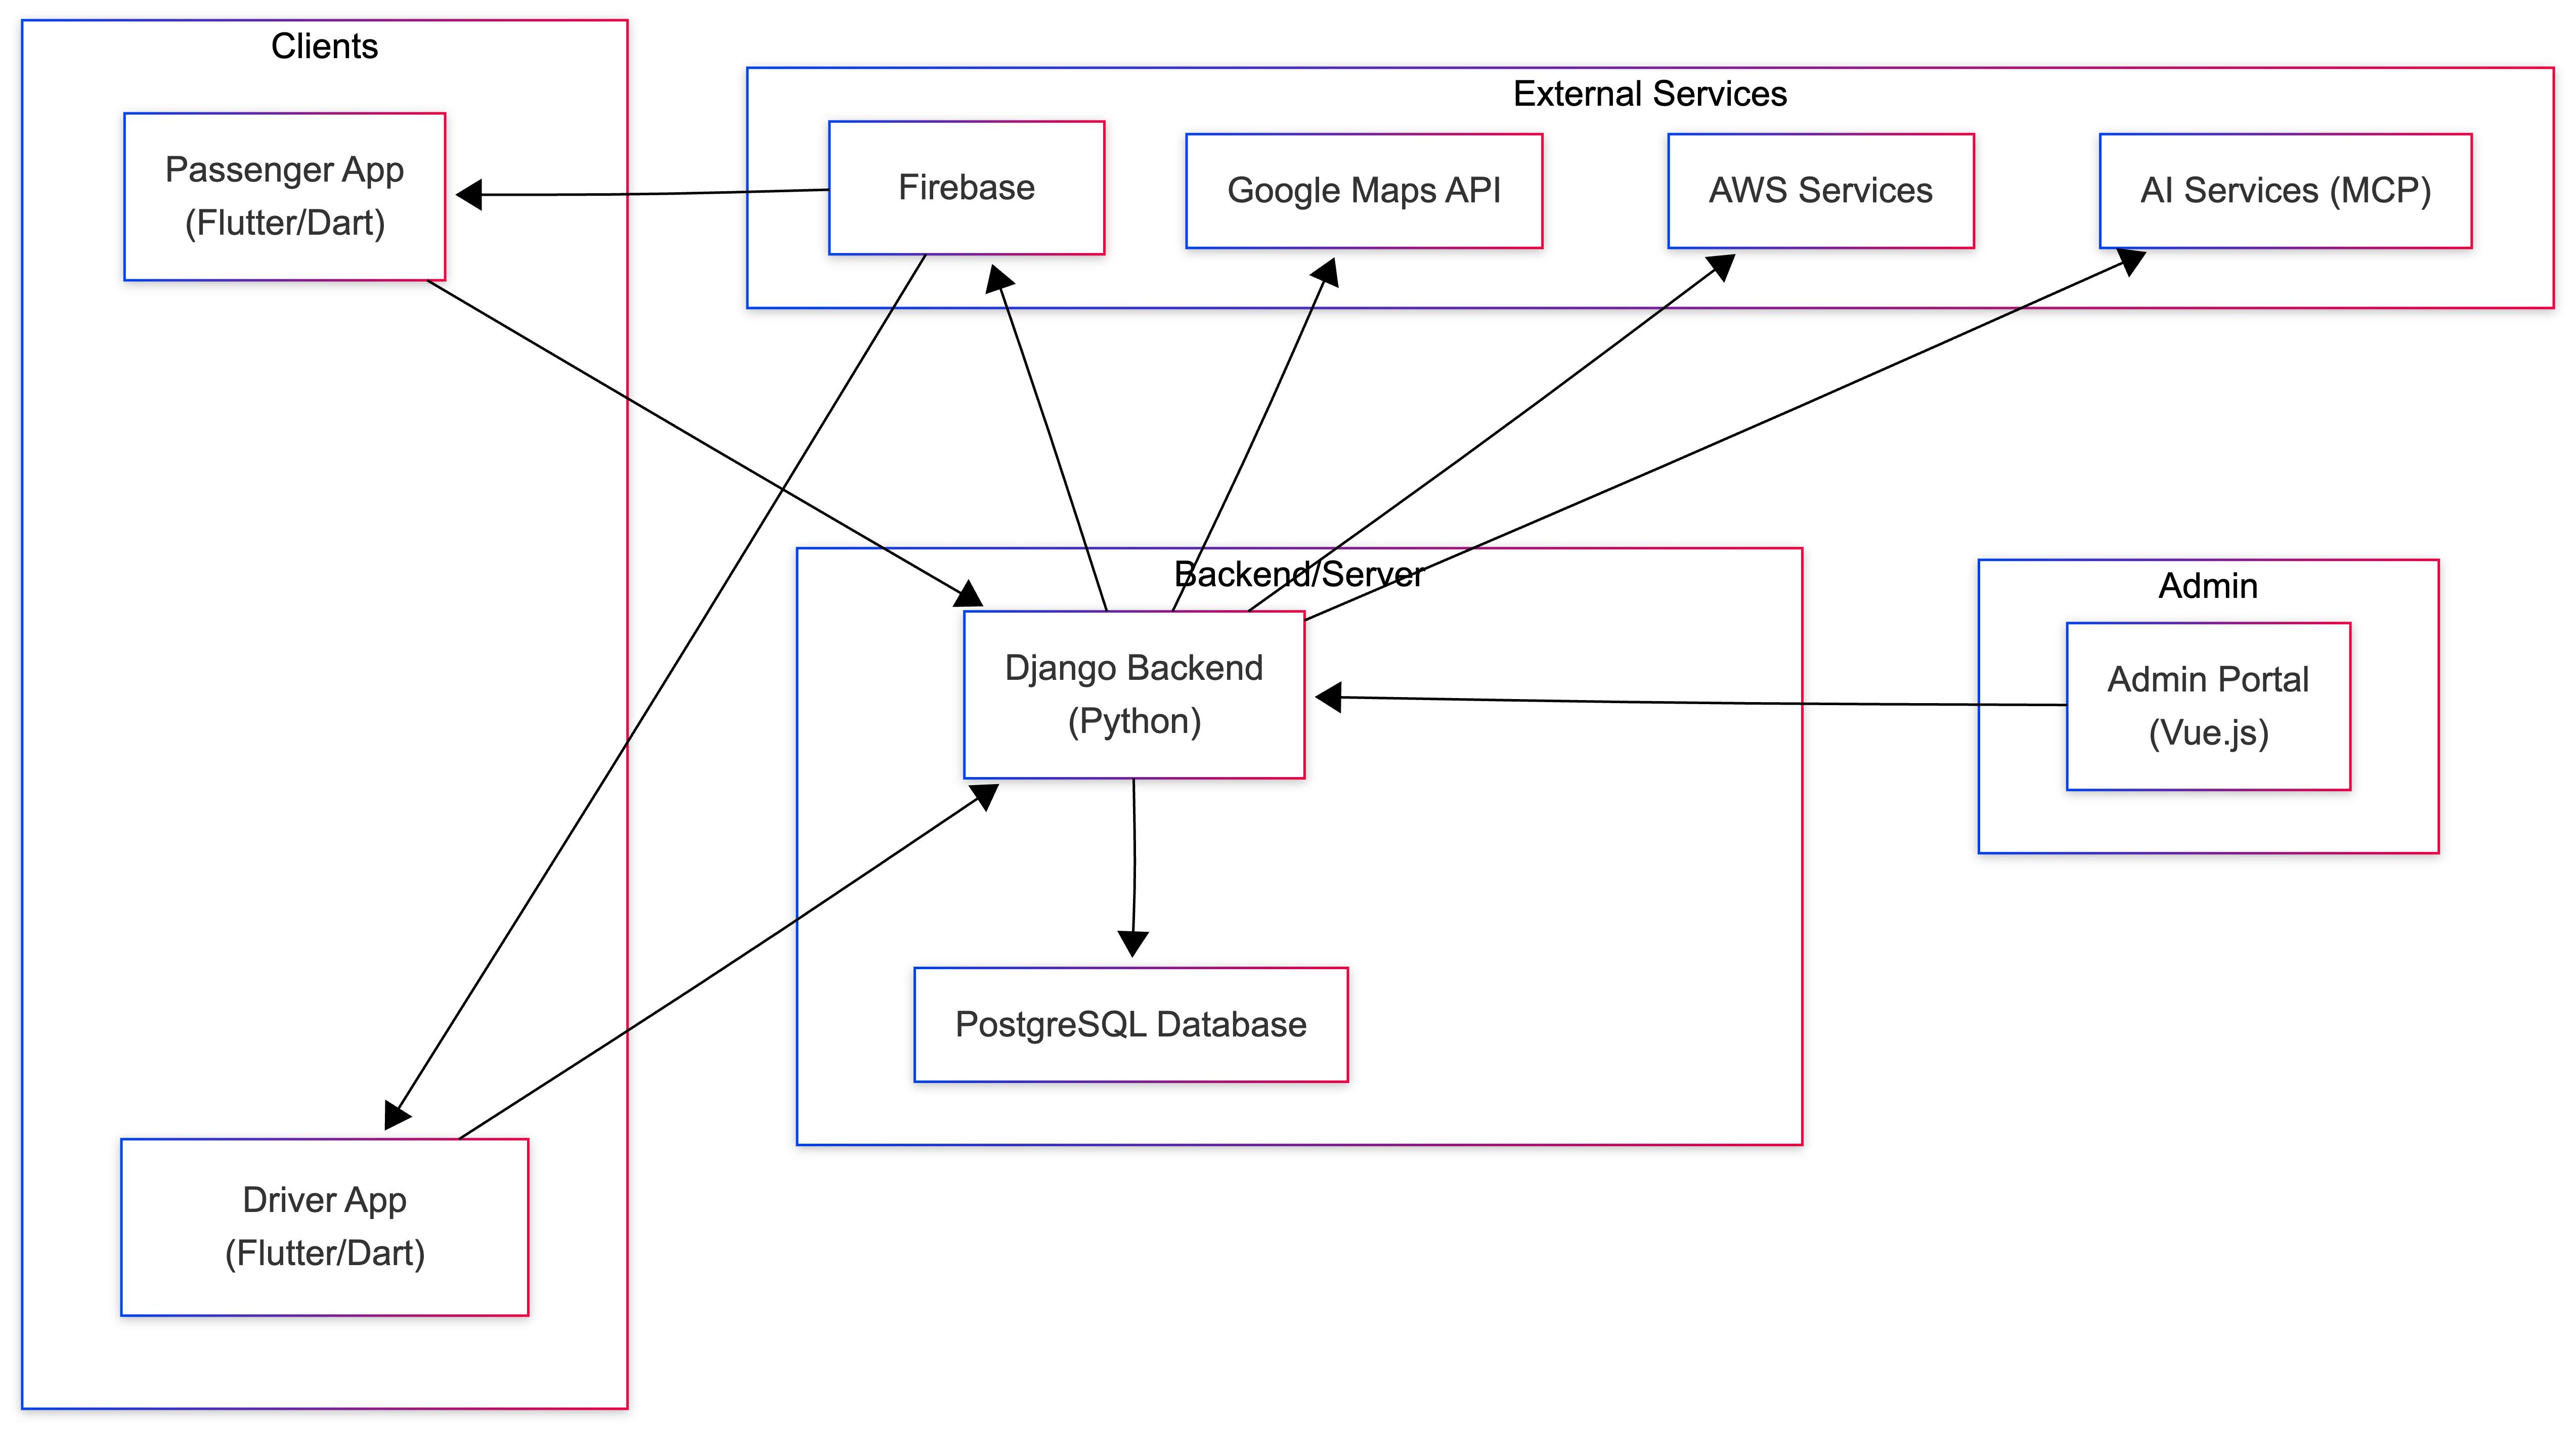
\includegraphics[width=0.8\textwidth]{images/methodology_2.png}
\caption{Methodology diagram of the entire system flow}
\label{fig:methodology}
\end{figure}

\subsection{Implementation}

The Traxis system was developed using an Agile-inspired iterative approach, structured around three focused sprints of approximately 3–4 weeks each. This methodology ensured continuous feedback, early delivery of functional components, and adaptability to evolving requirements. Development of the Passenger and Driver applications was performed from a single Flutter codebase, guaranteeing 100\% feature parity and identical behavior on both Android and iOS platforms from the outset.

\begin{itemize}
    \item \textbf{Sprint 1 – Foundation (Weeks 1–4)} \\
          The first sprint established the core infrastructure of the system. This included:
          \begin{itemize}
              \item Backend scaffolding with \textbf{Django} and \textbf{Django REST Framework}, creating the initial API endpoints and authentication logic.
              \item Database setup with \textbf{PostgreSQL} and the \textbf{PostGIS} extension, supporting geospatial queries for future ride matching and route calculations.
              \item Integration of \textbf{Firebase Authentication} for secure phone-number-based login and \textbf{Cloud Messaging} for real-time notifications.
              \item Implementation of the real-time location pipeline to track passenger and driver positions efficiently.
              \item Initial setup of \textbf{MCP (Model Control Plane)} for AI service integration, preparing APIs for future predictive ride matching and AI-based recommendations.
              \item Configuration of \textbf{AWS services} for compute-intensive tasks such as transcription, batch processing, and AI computations.
          \end{itemize}

    \item \textbf{Sprint 2 – Core Interaction (Weeks 5–8)} \\
          The second sprint focused on user-facing functionality and real-time interactions:
          \begin{itemize}
              \item Development of \textbf{Passenger and Driver UI components} using Flutter, including ride request flows, driver availability status, and passenger booking screens.
              \item Implementation of phone-number login with OTP verification, leveraging Firebase Authentication.
              \item Driver availability broadcasting and passenger request handling via the backend and Firebase Cloud Messaging.
              \item Aggressive local caching using \textbf{Hive} to maintain functionality in low-connectivity or intermittent network areas.
              \item Real-time push notifications for ride status updates and driver-passenger communication.
              \item Integration of MCP-based AI features into core flows, including predictive driver matching and demand forecasting, communicating via backend APIs.
              \item Offloading heavy processing tasks to AWS services, such as voice-to-text transcription for ride requests.
          \end{itemize}

    \item \textbf{Sprint 3 – Polish \& Advanced Features (Weeks 9–12)} \\
          The third sprint added advanced features, optimization, and system polish:
          \begin{itemize}
              \item Heatmap visualization for demand prediction and operational insights, leveraging MCP AI analytics.
              \item Trip history and detailed ride analytics for passengers and drivers.
              \item Rating and feedback system to ensure service quality.
              \item Admin portal enhancements, including dispute resolution tools and reporting dashboards.
              \item Performance tuning for backend and mobile apps, including optimization of AWS-backed compute tasks and MCP API calls.
              \item Accessibility features, such as voice prompts for drivers, high-contrast UI modes, and intuitive navigation.
          \end{itemize}
\end{itemize}

This implementation plan ensured that core functionality was delivered early, enabling iterative testing and feedback while progressively integrating advanced AI features and cloud-based services. By following this structured Agile approach, the development team maintained high code quality, ensured system reliability, and supported rapid adaptation to emerging user and business needs.

\begin{figure}[h]
\centering
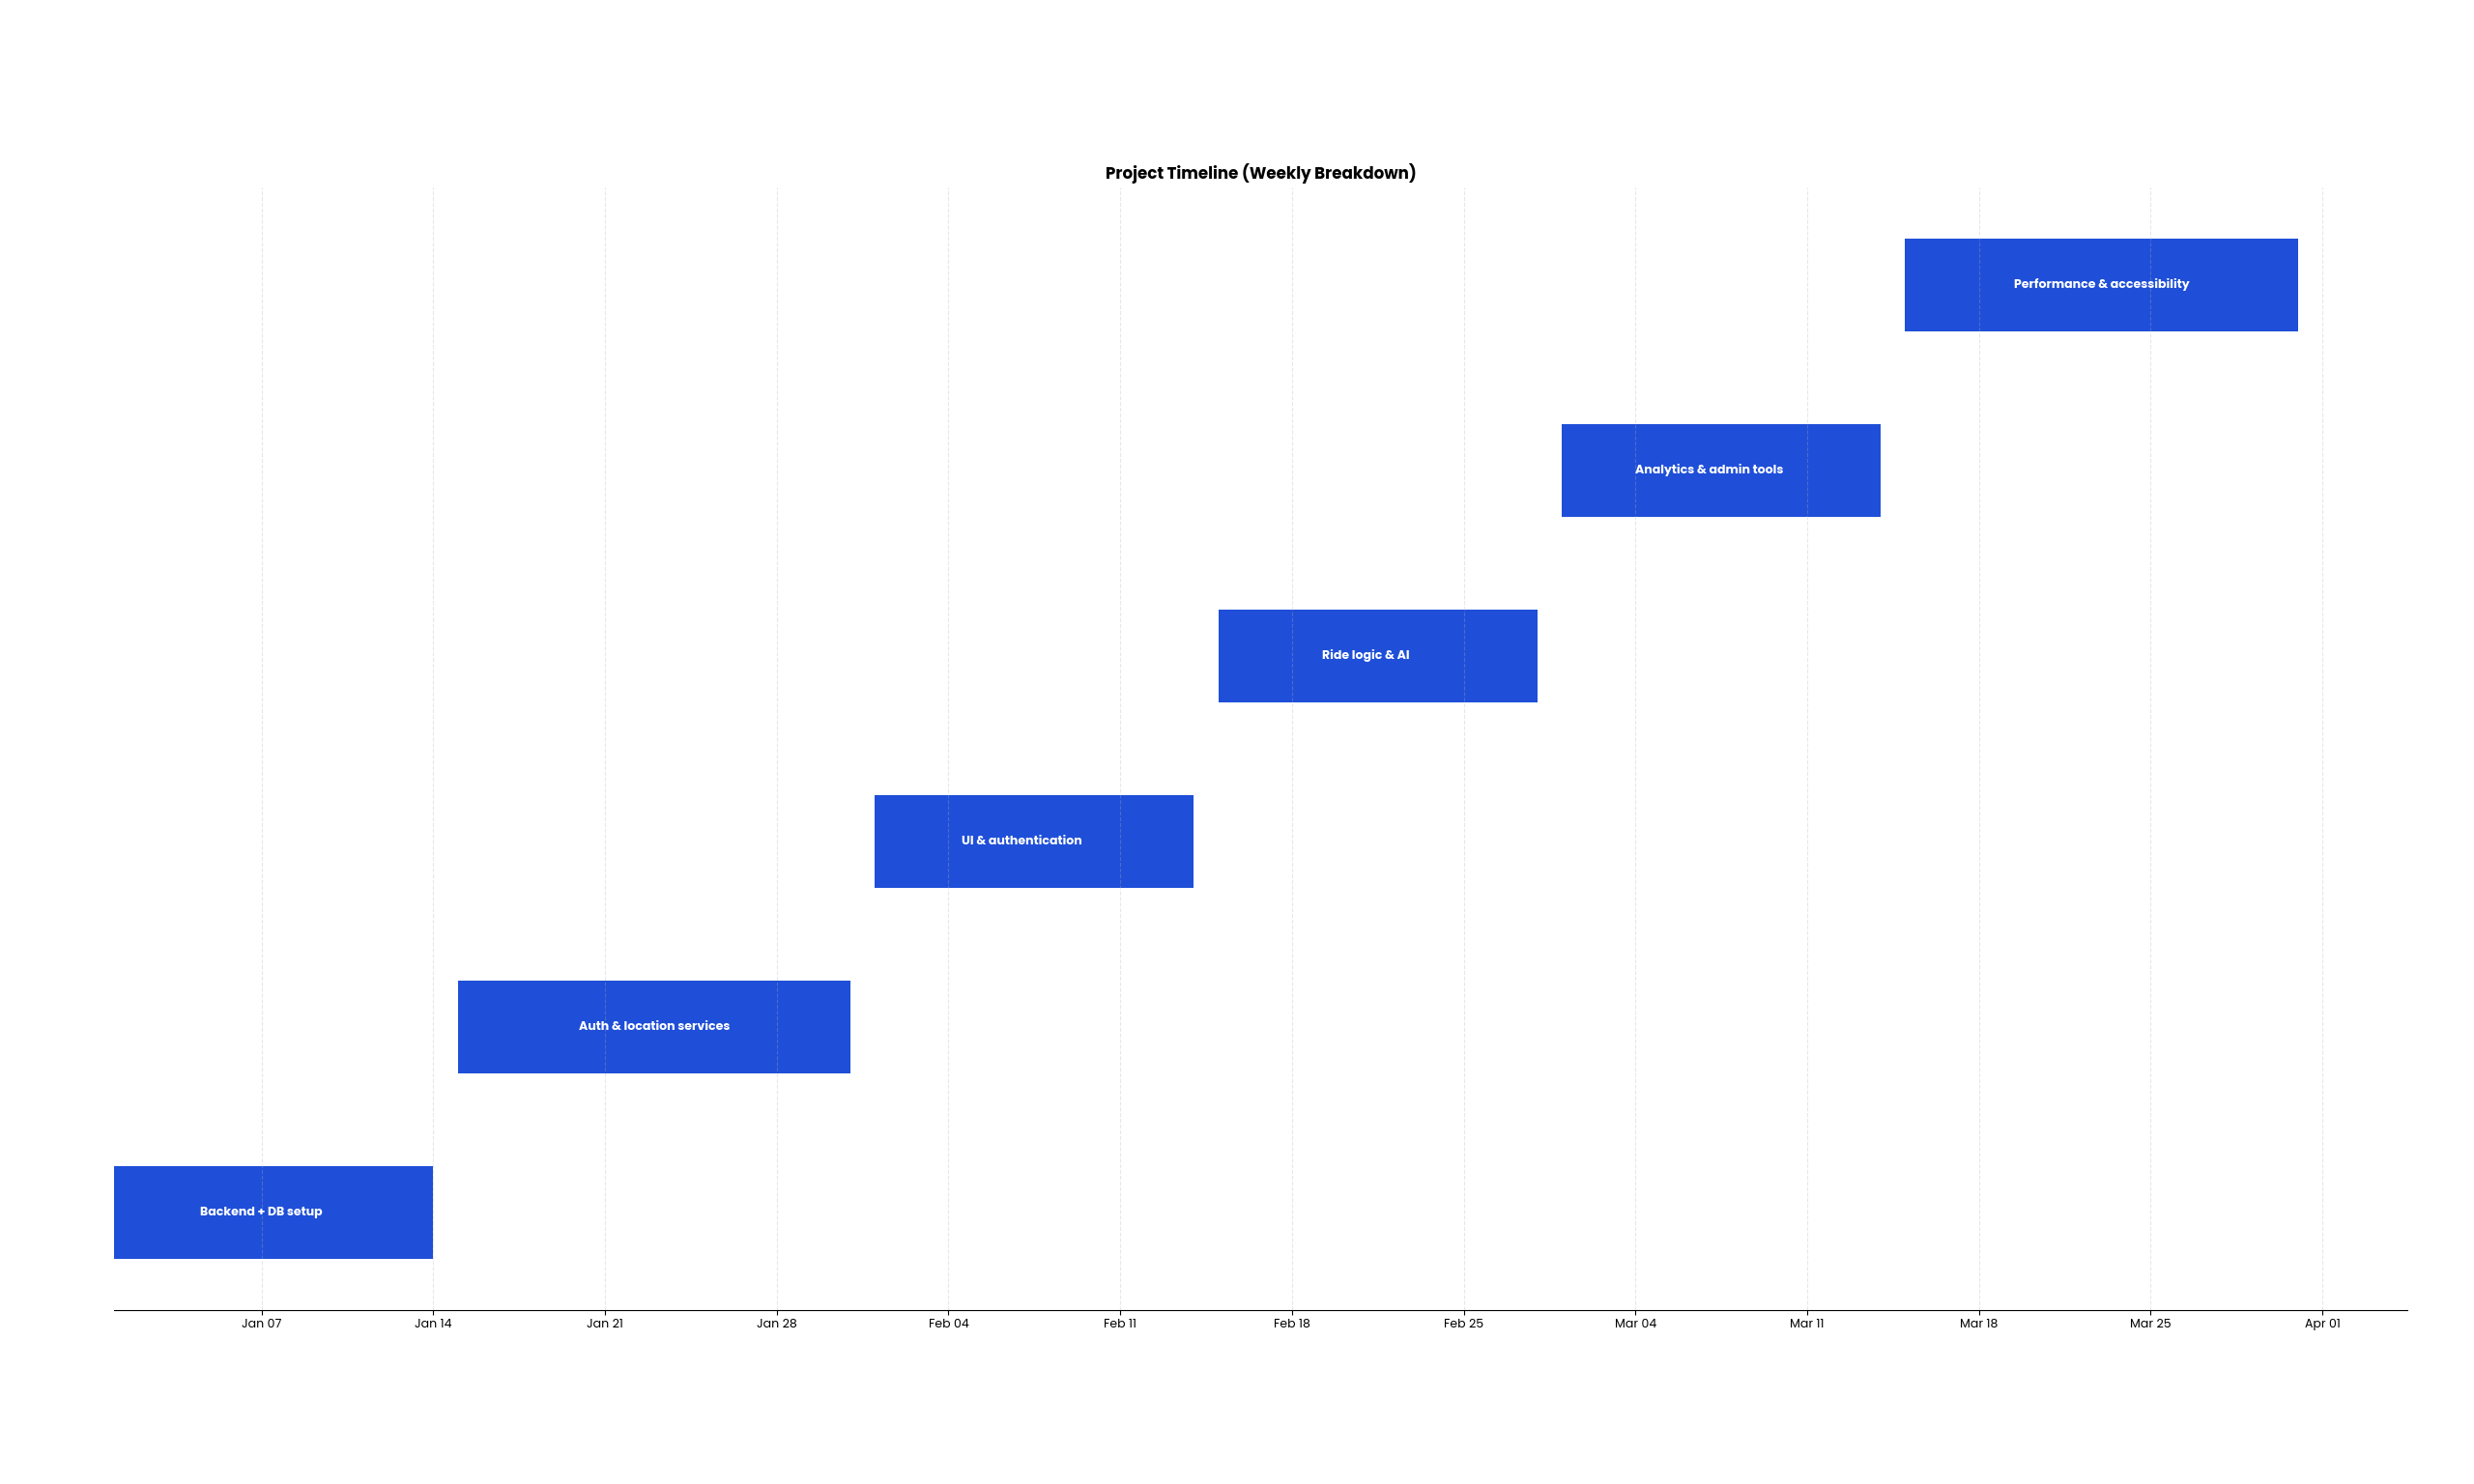
\includegraphics[width=1.05\textwidth]{images/gantt_2.png}
\caption{Gantt Chart showing the intended work plan}
\label{fig:gantt}
\end{figure}


\subsection{Project Management \& Version Control}

\textbf{Version Control: GitHub} \\
The project utilized GitHub for source code management and version control. A structured branching strategy was employed, including a \texttt{main} branch for production-ready code and a \texttt{develop} branch for ongoing development. All feature additions, bug fixes, and improvements were implemented through pull requests (PRs), which underwent code review before merging. This approach ensured code quality, traceability, and collaborative development while minimizing integration errors.

\textbf{Project Management: ClickUp} \\
ClickUp was used to plan, track, and manage all project activities. The platform supported the Agile sprint structure with task assignments, deadlines, and progress tracking through burndown charts. Automated reminders and notifications helped prevent task slippage, ensuring timely completion of features and alignment with the overall project timeline. Additionally, ClickUp provided transparency and accountability for all team members, facilitating efficient communication and coordination throughout the project lifecycle.
